\chapter{Specifiche Software}
In questo capitolo vengono descritte le specifiche software del sistema di posizionamento SFA. Si evidenziano le caratteristiche architetturali dei software che concorrono al raggiungimento dello scopo del sistema, e se ne descrivono i protocolli di comunicazione.
\section{Architettura Software}
Sulla piattaforma di elaborazione dati \`e installato il sistema operativo \texttt{Ubuntu 16.04 LTS}, basato su kernel \texttt{Linux}.
\\*
Su tale piattaforma viene eseguito il modulo SFA, opportunamente incapsulato in un eseguibile, denominato \texttt{listener}.\\*
Un set di moduli software, denominati \texttt{interface-modules}, sono in esecuzione sulla scheda. Lo scopo di questo insieme di programmi \`e quello di funzionare come interfaccia interna verso i sensori del CPS. 
La comunicazione fra \texttt{interface-modules} e \texttt{listener} avviene attraverso un protocollo applicazione stabilito arbitrariamente, sia esso \texttt{INPUT\_PROTOCOL}, mentre a livello di trasporto si utilizza \texttt{UDP}.\\*
I valori ricevuti da \texttt{listener} vengono salvati in apposite \emph{strutture dati} rappresentanti misure della stessa sorgente:
\begin{itemize}
\item I vettori accelerazione e velocit\`a angolare rilevati da IMU vengono convertiti nella struttura dati \texttt{IMU\_POD};
\item La velocit\`a rilevata dal Radar/Odometro viene convertita nella struttura dati \texttt{ODO\_POD};
\item La posizione rilevata dal GPS viene infine convertita nella struttura dati \texttt{GPS\_POD}.
\end{itemize}
Il software \texttt{listener} \`e in grado di inviare le misurazioni ricevute da \texttt{interface-modules} a SFA, quali variabili di tipo \texttt{IMU\_POD, ODO\_POD, GPS\_POD} ed altres\'i di ricevere la stima della posizione del treno, essendo questo l'output dell'algoritmo, quale variabile di tipo \texttt{SFA\_OUTPUT\_POD}.\\*
Ogniqualvolta \texttt{listener} riceva un' uscita da SFA, si fa carico della comunicazione tra scheda e OBCU, utilizzando un protocollo arbitrario a livello applicazione, sia esso \texttt{OUTPUT\_PROTOCOL}.\\*
Uno schema dell'architettura software \`e quello mostrato in figura \ref{fig:tdiagramint}.\\*
\begin{figure}[h]
	\centering
	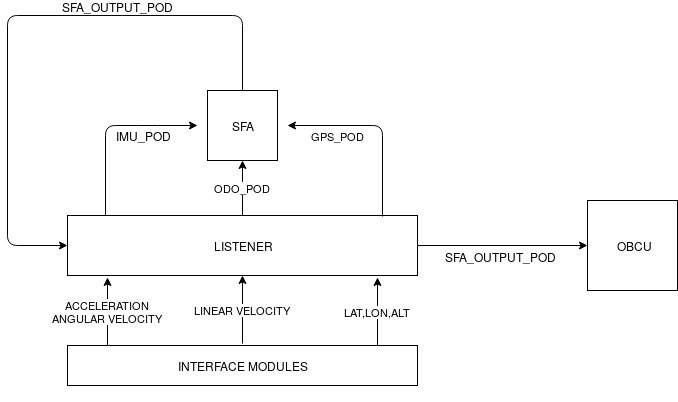
\includegraphics[width=\linewidth]{img/InternalTrainSchema}
	\caption{Architettura software bordo treno}
	\label{fig:tdiagramint}
\end{figure}
\section{Protocolli di Comunicazione}
Nella precedente sezione sono stati brevemente introdotti i protocolli di comunicazione implementati per gestire la comunicazione \texttt{UDP}:
\begin{itemize}
	\item In entrata, tra \texttt{interface-modules} e \texttt{listener} (\texttt{INPUT\_PROTOCOL});
	\item In uscita, tra \texttt{listener} e OBCU (\texttt{OUTPUT\_PROTOCOL}).
\end{itemize}
\subsection{Trasmissione in entrata}
Per trasmettere i dati da \texttt{interface-modules} a \texttt{listener}, e dunque dai sensori al modulo software che implementa SFA, \`e stato realizzato un protocollo di comunicazione denominato \texttt{INPUT\_PROTOCOL}.\\*
Tale protocollo fa affidamento a livello trasporto su \texttt{UDP} per massimizzare la velocit\`a di trasmissione.\\*
Il protocollo definisce il formato del \emph{payload} del pacchetto \texttt{UDP} che contiene le informazioni di IMU, Radar/Odometro, o GPS, ed \`e descritto in tabella \ref{tab:protoin}.\\*
\begin{table}[h]
			\centering
\begin{tabular}{|c|c|c|c|}
	\hline 
	\textbf{Campo} & \textbf{Descrizione} & \textbf{Indici di bit} & \textbf{Tipo} \\ 
	\hline 
	\texttt{SENSOR\_TYPE} & ID Sensore Sorgente & 0-7 & \texttt{uint8\_t} \\ 
	\hline 
	\texttt{Seq.NO} & Numero di sequenza & 8-23 & \texttt{uint16\_t} \\ 
	\hline 
	\texttt{N\_INT} & Numero di interi trasmessi & 24-31 & \texttt{uint8\_t} \\ 
	\hline 
	\texttt{N\_DOUBLE} & Numero di double trasmessi & 31-38 & \texttt{uint8\_t} \\ 
	\hline 
\end{tabular} 
\caption{Protocollo di comunicazione in entrata}
\label{tab:protoin}
\end{table}
A discrezione del valore del campo \texttt{SENSOR\_TYPE} si distingue il tipo di informazione trasportata dal pacchetto, come descritto in tabella \ref{tab:sensors}.\\*
\begin{table}[h]
		\centering
	\begin{tabular}{|c|c|}
		\hline 
		\textbf{Valore di SENSOR\_TYPE} & \textbf{Sorgente del pacchetto} \\ 
		\hline 
		$1$ & IMU \\ 
		\hline 
		$2$ & ODOMETRO \\ 
		\hline 
		$3$ & GPS \\ 
		\hline 
		$8$ & GROUND TRUTH \\ 
		\hline 
		$9$ & STROBE \\ 
		\hline 
		$10$ & STOP \\ 
		\hline 
	\end{tabular} 
	\caption{Significato del campo SENSOR\_TYPE}
	\label{tab:sensors}
\end{table}
I pacchetti \texttt{GROUND TRUTH} sono pacchetti di inizializzazione dell'algoritmo: alla ricezione del pacchetto \texttt{GROUND TRUTH} l'algoritmo si avvia leggendo i valori trasmessi in coda al pacchetto, in accordo al valore dei campi \texttt{N\_INT} e \texttt{N\_DOUBLE}. Tali valori forniscono informazioni come progressiva chilometrica e velocit\`a iniziali del treno.\\*
I pacchetti \texttt{STROBE} sono inviati ogni secondo e forniscono un solo valore \texttt{double}, ossia un \emph{timestamp} che l'algoritmo utilizza per sincronizzarsi. Per quanto esposto nel Capitolo 2, l'interfaccia \texttt{UDP} attraverso cui comunicano \texttt{interface-modules} e \texttt{listener} funge da TSI per il sistema.\\*
Il pacchetto \texttt{STOP} non contiene alcuna informazione utile: indica soltanto all'algoritmo di terminare l'esecuzione.\\*
Alla ricezione di un pacchetto, \texttt{listener} legge il valore del campo\\*\texttt{SENSOR\_TYPE}, e costruisce, in accordo alla relazione sorgente-struttura dati, la variabile da inviare a SFA.\\*
Il corretto ordinamento dei pacchetti trasmessi a SFA \`e garantito attraverso l'esplicito utilizzo di un buffer, codificato all'interno di \texttt{listener}, in cui i pacchetti vengono temporaneamente salvati prima di essere inviati a SFA, ed eventualmente ordinati sulla base del valore del campo \texttt{Seq.NO}.\\*
Si osservi che \texttt{UDP} non garantisce che l'ordine dei messaggi ricevuti sia lo stesso con i quali essi sono stati inviati. I messaggi potrebbero essere soggetti a ritardi casuali in base allo stato del sistema operativo. Utilizzando \texttt{TCP} si ovvierebbe a questa problematica, ma l'overhead insito nel protocollo stesso causerebbe un notevole degrado delle performance di SFA.
\subsection{Trasmissione in uscita}
La trasmissione dei dati in uscita da SFA avviene, in accordo al protocollo \texttt{OUTPUT\_PROTOCOL} tra \texttt{listener} e OBCU.\\*
Come specificato, la comunicazione \`e posta in essere, a livello fisico, attraverso il protocollo \texttt{LTE}, mentre a livello trasporto si \`e scelto di continuare a usare \texttt{UDP} in luogo di \texttt{TCP}, col fine di massimizzare le \emph{performance} del sistema. Il conseguente rischio di ricevere alcuni messaggi in maniera errata, o non riceverli del tutto, \`e tanto pi\`u elevato quanto l'ambiente entro cui si propaga fisicamente la radiazione elettromagnetica \`e pi\`u disturbato da sorgenti esterne e corpi fisici interposti.\\*
Questa problematica \`e risolta a livello software, attraverso l'esplicito utilizzo di un meccanismo di \texttt{acknowledgment} simile a quello utilizzato da \texttt{TCP}: ciascun pacchetto in uscita da SFA viene indicizzato con un \emph{sequence number} e, in ricezione, viene inviato ogni secondo un \emph{ack} replicante l'ultimo numero di sequenza correttamente ricevuto.
Anche in questo caso, il protocollo definisce il formato del \emph{payload} del pacchetto \texttt{UDP} inviato da \texttt{listener}, ed \`e riportato in tabella \ref{tab:protoout}.\\*
\begin{table}[h]
	\centering
	\begin{tabular}{|c|c|c|c|}
		\hline 
		\textbf{Campo} & \textbf{Descrizione} & \textbf{Indici di bit} & \textbf{Tipo} \\ 
		\hline
		\texttt{Seq.NO} & Numero di sequenza & 0-15 & \texttt{uint16\_t} \\ 
		\hline 
		\texttt{Epoch} & Timestamp & 16-79 & \texttt{double} \\ 
		\hline 
		\texttt{FU\_ARC\_LEN} & Progressiva chilometrica & 80-143 & \texttt{double} \\ 
		\hline 
		
	\end{tabular} 
\caption{Protocollo di comunicazione in uscita}
\label{tab:protoout}
\end{table}
\clearpage
In ricezione, OBCU dovr\`a inviare un pacchetto \emph{ack} al mittente, ed il suo formato \`e descritto in tabella \ref{tab:ack}.
\begin{table}[h]
	\centering
	\begin{tabular}{|c|c|c|c|}
	\hline 
	\textbf{Campo} & \textbf{Descrizione} & \textbf{Indici di bit} & \textbf{Tipo} \\ 
	\hline
	\texttt{ACK} & Ultimo \texttt{Seq.NO} & 0-15 & \texttt{uint16\_t} \\ 
	\hline
\end{tabular}
\caption{Formato del pacchetto di \emph{ack}}
\label{tab:ack}
\end{table}
Si osservi che, ai fini del posizionamento, l'ordinamento dei pacchetti ricevuti non \`e fondamentale. A differenza di quanto esposto nel caso della trasmissione dei dati in entrata a SFA, \`e sufficente che OBCU faccia riferimento al messaggio con il \emph{timestamp} pi\`u recente.
\section{Scenario di Esempio}
Si suppongano le condizioni iniziali riportate in tabella \ref{tab:condinit}.\\*
\begin{table}[h]
	\centering
	\begin{tabular}{|c|c|c|c|c|}
		\hline 
		\textbf{Vettore Velocit\`a} & \textbf{Progressiva} & \textbf{IMU Sample Rate} & \textbf{ODO Sample Rate} \\ 
		\hline 
		$(0.0, 0.0, 0.0) ms^{-1}$ & 0 km & 100 Hz & 20 Hz \\ 
		\hline 
	\end{tabular} 
	\caption{Condizioni iniziali}
	\label{tab:condinit}
\end{table}
\begin{enumerate}
	\item $t = 0$:\\*
	\begin{itemize}
	\item \texttt{interface-modules} invia a \texttt{listener} il seguente pacchetto \texttt{GROUND TRUTH}:\\*\\*
	\begin{tabular}{|c|c|c|c|}
		\hline 
		\textbf{SENSOR\_TYPE} & \textbf{Seq. NO} & \textbf{N\_INT} & \textbf{N\_DOUBLE} \\ 
		\hline 
		\texttt{0x08} & \texttt{0x00} & 0 & 4 \\ 
		\hline 
	\end{tabular}\\*\\*
	E vi accoda i seguenti tre valori \texttt{double: 0.0, 0.0, 0.0}, ossia il vettore velocit\`a iniziale, ed il valore \texttt{double 0.0}, che rappresenta la progressiva chilometrica iniziale.
	\item \texttt{listener} riceve il pacchetto e inizializza SFA con:
	\begin{itemize}
		\item Velocit\`a iniziale: $(0, 0, 0)$
		\item Progressiva chilometrica iniziale: $0.0$
	\end{itemize}
	\end{itemize}
	\newpage
	\item $t=t_0$:\\*
	\begin{itemize}
	\item IMU campiona il seguente vettore accelerazione:
	$$
	\mathbf{a} = (0.0001, -0.0001, -9.8100)
	$$
	Assieme al seguente vettore velocit\`a angolare:
	$$
	\mathbf{v_{ang}} = (0.0003, -0.0001, 0.0002)
	$$
	Il pacchetto viene inviato a \texttt{interface-modules} attraverso i bus dati, e conseguentemente:
	\item \texttt{interface-modules} invia a \texttt{listener}, attraverso la socket \texttt{UDP}, il seguente pacchetto \texttt{IMU}:\\*\\*
		\begin{tabular}{|c|c|c|c|}
		\hline 
		\textbf{SENSOR\_TYPE} & \textbf{Seq. NO} & \textbf{N\_INT} & \textbf{N\_DOUBLE} \\ 
		\hline 
		\texttt{0x01} & \texttt{0x01} & 0 & 6 \\ 
		\hline 
	\end{tabular}\\*\\*
	Accodandovi nell'ordine il vettore accelerazione, e il vettore velocit\`a angolare.
	\item \texttt{listener} riceve il pacchetto, crea e inoltra a SFA la seguente variabile \texttt{IMU\_POD}:
	\begin{itemize}
		\item \texttt{Seq.NO = 1}
		\item \texttt{Epoch = $t_0$}
		\item \texttt{ACC\_X = 0.0001}
		\item \texttt{ACC\_Y = -0.0001}
		\item \texttt{ACC\_Z = -9.8100}
		\item \texttt{GYRO\_X = 0.0003}
		\item \texttt{GYRO\_Y = -0.0001}
		\item \texttt{GYRO\_Z = 0.0002}
	\end{itemize}
\item SFA elabora i dati ricevuti e inizia una computazione parallela per fornire a \texttt{listener} una variabile \texttt{SFA\_OUTPUT\_POD} della forma:
	\begin{itemize}
		\item \texttt{Seq.NO = 0}
		\item \texttt{FU\_ARC\_LEN = }$P_{KM}$
	\end{itemize}
	\end{itemize}
	\item $t_0 < t < t_0 + \frac{1}{ODO\_SAMPLE\_RATE} = t_0 + \frac{1}{20}$\\*
	Fintantoch\'e l'odometro non campiona il suo primo valore di velocit\`a, si ripetono le operazioni viste al passo precedente per ogni campionamento di \texttt{IMU}.
	\item $t = t_0 + \frac{1}{20}$\\*
		\begin{itemize}
		\item Odometro campiona, e invia a \texttt{interface-modules}, il seguente valore di velocit\`a:
		$$
		v = (1.0010)
		$$
		\texttt{interface-modules} invia a \texttt{listener} il seguente pacchetto \texttt{ODOMETRO}:\\*\\*
		\begin{tabular}{|c|c|c|c|}
			\hline 
			\textbf{SENSOR\_TYPE} & \textbf{Seq. NO} & \textbf{N\_INT} & \textbf{N\_DOUBLE} \\ 
			\hline 
			\texttt{0x02} & \texttt{Seq\_{NO}} & 0 & 2 \\ 
			\hline 
		\end{tabular}\\*\\*
		Accodandovi nell'ordine il valore di velocit`a rilevato, e il valore dello scarto quadratico medio della sorgente, noto a priori, in quanto caratteristica tecnica intrinseca dello strumento di misura, il radar; sia esso \texttt{SIGMA\_{RADAR}}.\\*
		\item \texttt{listener} riceve il pacchetto, crea e invia a SFA la seguente variabile \texttt{ODO\_POD}:
		\begin{itemize}
			\item \texttt{Seq.NO = Seq\_{NO}}
			\item \texttt{Epoch = $t_0 + \frac{1}{20}$}
			\item \texttt{vel = 1.0010}
			\item \texttt{sigma = SIGMA\_{RADAR}}
		\end{itemize}
		\item SFA elabora i dati ricevuti e utilizza la rilevazione di velocit\`a in maniera utile a migliorare la stima della posizione.
		\end{itemize}
	\item $t = n\;t_0\;\;\;\;\;\;\;n \in \mathbb{N}^+$\\*
	Ogni secondo, il modulo \texttt{STROBE} di \texttt{interface-modules}, invia a \texttt{listener} un pacchetto della forma:
	\\*\\*
	\begin{tabular}{|c|c|c|c|}
		\hline 
		\textbf{SENSOR\_TYPE} & \textbf{Seq. NO} & \textbf{N\_INT} & \textbf{N\_DOUBLE} \\ 
		\hline 
		\texttt{0x09} & \texttt{Seq\_{NO}} & 0 & 1 \\ 
		\hline 
	\end{tabular}\\*\\*
Accondandovi un \emph{timestamp} che \texttt{listener} inoltra a SFA per scopi di sincronizzazione.
\end{enumerate}
Quanto elencato viene ripetuto per ciascun campionamento successivo di IMU e odometro.\\*
Nonappena la prima uscita di SFA si rende disponibile a \texttt{listener} questo si comporta come segue:
\begin{itemize}
	\item \texttt{listener} riceve la variabile \texttt{SFA\_OUTPUT\_POD}, da SFA;
	\item Supponendo di trovarsi al tempo $T$, \texttt{listener} costruisce ed invia ad OBCU il seguente pacchetto:\\*\\*
		\begin{tabular}{|c|c|c|}
		\hline 
		\textbf{Seq. NO} & \textbf{Epoch} & \textbf{FU\_ARC\_LEN} \\ 
		\hline 
		\texttt{0x00} & $T$ & $P_{KM_T}$ \\ 
		\hline 
	\end{tabular}\\*\\*
	\item OBCU riceve il pacchetto e invia a \texttt{listener} l'\emph{ack} \texttt{0x00}.
\end{itemize}
